\subsection{Hậu Quả Khi Vi Phạm Tuyến Tính}
% -----------------------------------------------------------------------------

Khi dạng hàm thực là phi tuyến nhưng ta khớp bằng đường thẳng, đường thẳng đó hấp thụ độ cong vào hệ số, tạo ra trung bình \textit{sai ở mọi nơi}---không chỉ ồn ào mà là chệch có cấu trúc. Đây là vi phạm nguy hiểm nhất vì nó phá vỡ tính không chệch ngay tại lõi của OLS. Năm biểu hiện quan sát được:

\textbf{1. Ước lượng chệch:} $E[\hat{\beta}] \neq \beta$---hệ số sai trung bình, không phải chỉ không chính xác. OLS hấp thụ phần phi tuyến bị bỏ sót vào hệ số, làm lệch ước lượng tốc độ thay đổi của biến phản hồi.

\textbf{2. Mẫu hình phần dư có hệ thống:} đồ thị phần dư theo giá trị khớp cho thấy dạng cong (chữ U, chữ S) thay vì phân tán ngẫu nhiên---đây là tín hiệu chẩn đoán chính. Đường LOESS lệch khỏi $y = 0$ một cách có quy luật.

\textbf{3. Khớp kém:} $s^2$ bị thổi phồng vì mô hình quy cho sai số ngẫu nhiên những phần biến động thực ra có cấu trúc. Khoảng tin cậy quá rộng, kiểm định mất sức mạnh thống kê.

\textbf{4. Suy diễn không hợp lệ:} kiểm định $t$ và $F$ dựa trên mô hình sai lệch---$p$-value và khoảng tin cậy không đáng tin. Một biến có thể có ý nghĩa thống kê không phải vì tác động thực, mà vì nó đang bù đắp cho phần phi tuyến bị thiếu.

\textbf{5. Dự báo không chính xác:} khoảng cách giữa đường khớp và đường cong thực mở rộng ra ngoài vùng huấn luyện, nơi ngoại suy nguy hiểm nhất.

\textbf{Điểm phân biệt quan trọng.} Khác với vi phạm giả định chuẩn tắc (chỉ ảnh hưởng đến suy diễn), vi phạm tuyến tính ảnh hưởng trực tiếp đến \textit{bản thân ước lượng $\hat{\beta}$} và $\hat{y}$: chúng không còn ước lượng đúng tham số quan tâm nữa.

\subsubsection{Tứ Giác Anscombe}

Anscombe (1973), được Weisberg dùng để nhấn mạnh vai trò của chẩn đoán phần dư \cite[Sec.~2.4, p.~27]{weisberg2014applied}, đã xây dựng bốn bộ dữ liệu có cùng $\hat{\beta}_0 \approx 3$, $\hat{\beta}_1 \approx 0.5$, $R^2 \approx 0.67$ và $p$-value---nhưng nhìn hoàn toàn khác nhau. Bộ~II rõ ràng là quan hệ bậc hai. Bộ~III bị một điểm ngoại lai kéo hệ số. Bộ~IV có đòn bẩy cực cao tại một điểm. Kết quả hồi quy không cảnh báo gì cả; chỉ đồ thị phần dư mới tiết lộ vi phạm.

\begin{figure}[H]
  \centering
  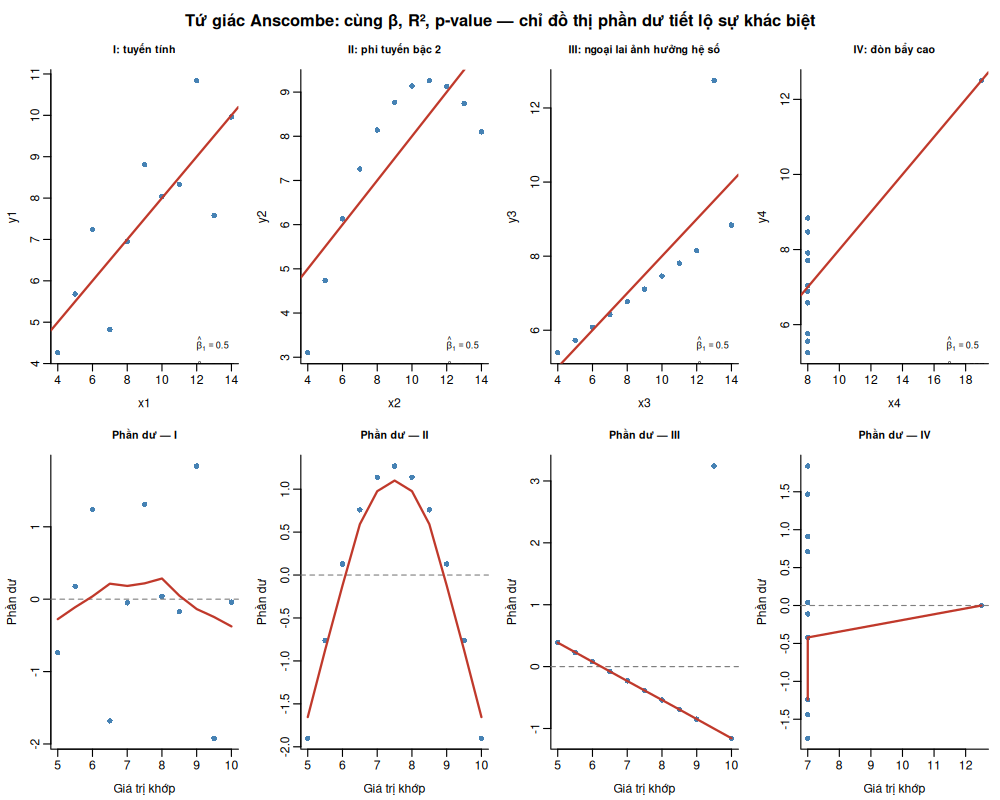
\includegraphics[width=\textwidth]{./figures/fig7_anscombe.png}
  \caption{Tứ giác Anscombe: bốn bộ dữ liệu với cùng $\hat{\beta}_1 \approx 0.5$ và $R^2 \approx 0.67$.
  \textbf{Hàng trên:} scatterplot với đường hồi quy bậc nhất---nhìn qua output số không phân biệt được.
  \textbf{Hàng dưới:} đồ thị phần dư theo giá trị khớp.
  Bộ~I (tuyến tính): phần dư ngẫu nhiên, LOESS nằm ngang.
  Bộ~II (phi tuyến bậc 2): LOESS cong hình cung, vi phạm tuyến tính rõ.
  Bộ~III (ngoại lai): một điểm kéo hệ số lên cao, phần dư có điểm ngoại lai lớn.
  Bộ~IV (đòn bẩy): một điểm kiểm soát toàn bộ hồi quy.}
  \label{fig:anscombe}
\end{figure}

\begin{lstlisting}[style=Rstyle]
data(anscombe)
# Tat ca co cung he so hoi quy va R2
fits <- lapply(1:4, function(i)
  lm(anscombe[[paste0("y",i)]] ~ anscombe[[paste0("x",i)]]))

do.call(rbind, lapply(fits, function(m) {
  s <- summary(m)
  round(c(b0 = coef(m)[1], b1 = coef(m)[2],
          R2 = s$r.squared, p = coef(s)[2,4]), 3)
}))
\end{lstlisting}

\begin{lstlisting}[style=output]
     b0    b1     R2     p
[1,] 3.00 0.500 0.667 0.002
[2,] 3.00 0.500 0.666 0.002
[3,] 3.00 0.500 0.666 0.002
[4,] 3.00 0.500 0.667 0.002
\end{lstlisting}

\subsubsection{Ví Dụ Thực Tế}

Bốn bộ dữ liệu từ các lĩnh vực khác nhau minh họa cùng một mẫu hình: đường thẳng OLS không bám sát dữ liệu, và đồ thị phần dư phản chiếu rõ độ cong bị bỏ sót.

\begin{figure}[H]
  \centering
  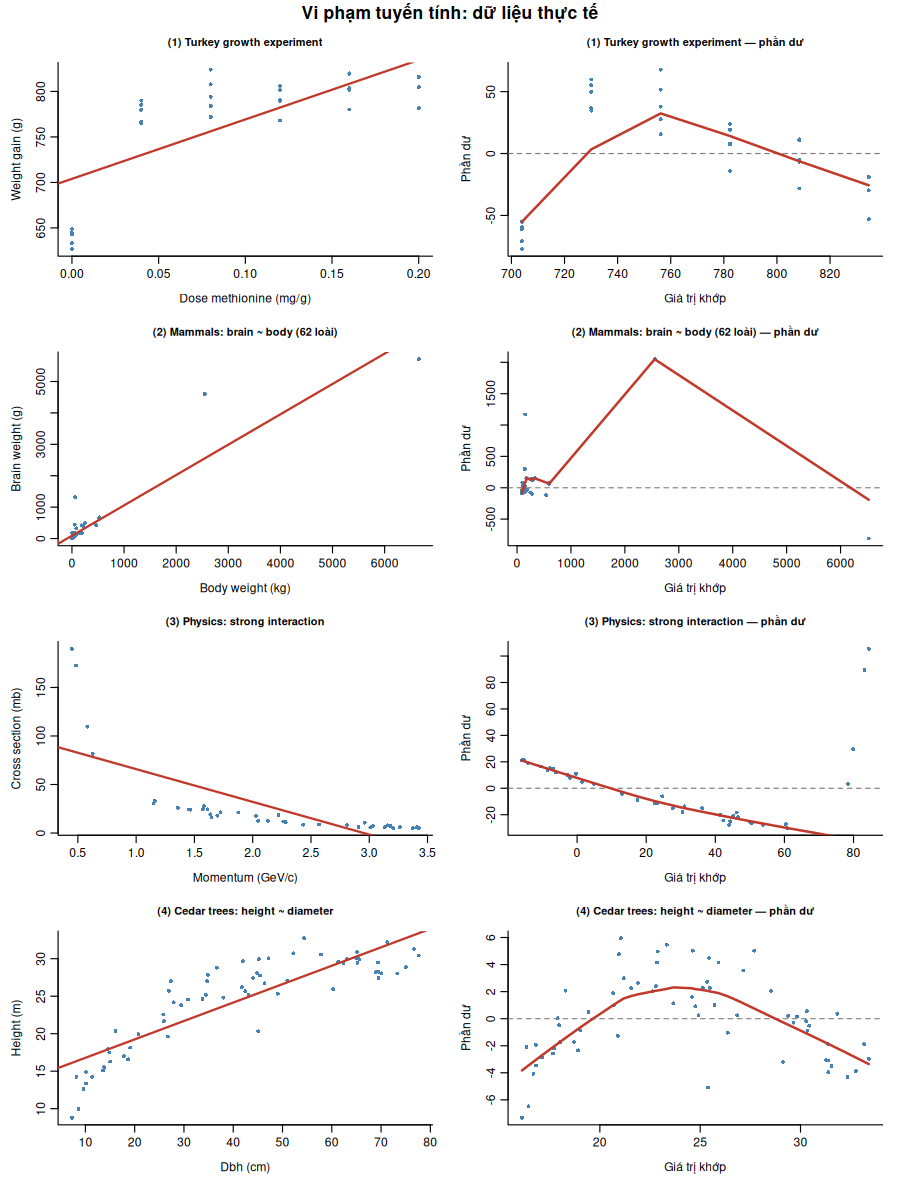
\includegraphics[width=\textwidth]{./figures/fig12_violations.png}
  \caption{Bốn ví dụ thực tế vi phạm tính tuyến tính.
  \textbf{Cột trái:} scatter plot với đường hồi quy OLS bậc 1 (đỏ).
  \textbf{Cột phải:} đồ thị phần dư theo giá trị khớp; đường LOESS (đỏ) lệch có hệ thống khỏi $y = 0$.
  \textbf{(1) Turkey growth:} tốc độ tăng cân theo liều methionine bão hòa dần---đường thẳng đánh giá thấp ở đầu, cao ở cuối.
  \textbf{(2) Mammals:} khối lượng não theo khối lượng cơ thể trải dài hàng nghìn lần---OLS bị chi phối bởi vài loài lớn.
  \textbf{(3) Physics:} tiết diện tán xạ giảm nhanh theo đà---dạng lũy thừa không thể khớp bằng đường thẳng.
  \textbf{(4) Cedar trees:} chiều cao cây tiệm cận mức tối đa khi đường kính lớn---dạng sigmoid.}
  \label{fig:violations}
\end{figure}

\begin{lstlisting}[style=Rstyle]
# -- (1) Turkey growth: E(Y|Dose) = b0 + b1*(1 - exp(-b2*Dose)) --------------
set.seed(101)
dose_lvl <- c(0, 0.04, 0.08, 0.12, 0.16, 0.20)
dose_t   <- rep(dose_lvl, each = 5)
y_turkey <- 639 + 168*(1 - exp(-37*dose_t)) + rnorm(30, 0, 18)

fit_lin_t <- lm(y_turkey ~ dose_t)
plot(dose_t, y_turkey, pch = 16, col = "steelblue",
     xlab = "Dose (mg/g)", ylab = "Weight gain (g)")
abline(fit_lin_t, col = "red", lwd = 2)
plot(fit_lin_t, which = 1)   # phan du cong ro

# -- (2) Mammals: brain ~ body (MASS) -----------------------------------------
library(MASS); data(mammals)
fit_raw <- lm(brain ~ body, data = mammals)
plot(fit_raw, which = 1)     # phan du bien dang nang

# -- (3) Physics cross sections ------------------------------------------------
set.seed(102)
x_phys <- sort(runif(38, 0.3, 3.5))
y_phys <- 45 * x_phys^(-1.7) * exp(rnorm(38, 0, 0.15))

fit_lin_p <- lm(y_phys ~ x_phys)
plot(fit_lin_p, which = 1)   # LOESS cong chu U

# -- (4) Cedar trees: height ~ dbh --------------------------------------------
set.seed(103)
dbh    <- sort(runif(65, 5, 78))
height <- 30*(1 - exp(-0.055*dbh)) + rnorm(65, 0, 2.2)

fit_lin_d <- lm(height ~ dbh)
plot(fit_lin_d, which = 1)   # LOESS cong chu S
\end{lstlisting}

Trong cả bốn trường hợp, đường LOESS trên đồ thị phần dư lệch khỏi $y = 0$ theo mẫu hình có hệ thống---dấu hiệu chẩn đoán chính của sai dạng hàm trung bình. Hình~\ref{fig:violations_fixed} minh họa các cách sửa khác nhau: log-log và spline vẫn có thể viết như mô hình tuyến tính theo tham số sau biến đổi hoặc sau khi dựng hàm cơ sở; riêng Turkey phải dùng NLS vì tham số $\beta_2$ nằm trong hàm mũ, nên đây là hồi quy phi tuyến theo tham số chứ không còn là OLS tuyến tính cổ điển.

\begin{figure}[H]
  \centering
  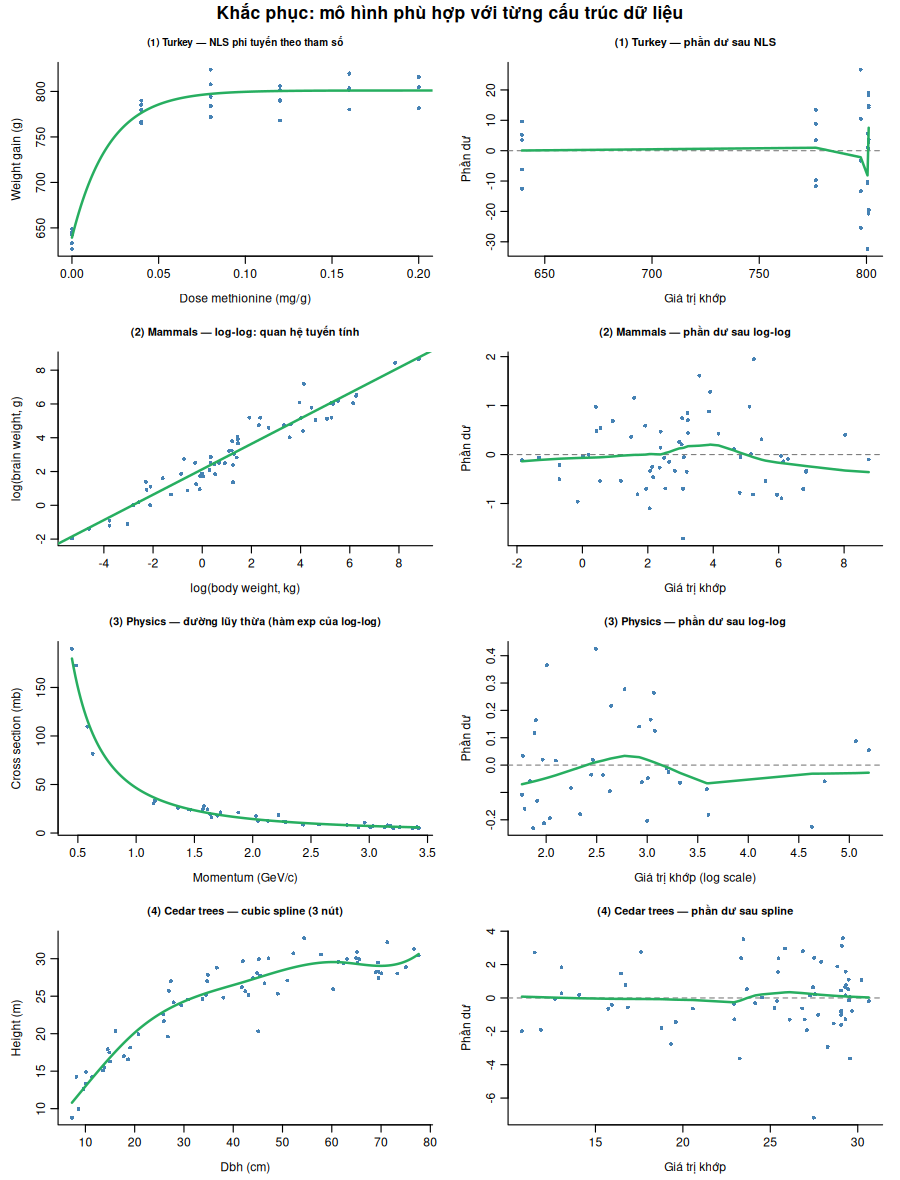
\includegraphics[width=\textwidth]{./figures/fig13_violations_fixed.png}
  \caption{Cùng bốn bộ dữ liệu sau khi sửa đặc tả hàm trung bình (xanh lá). Hình này không nói rằng mọi cách sửa vẫn thuộc OLS tuyến tính cổ điển.
  \textbf{(1) Turkey:} NLS với dạng bão hòa $\beta_0 + \beta_1[1 - e^{-\beta_2 \cdot \text{dose}}]$---phù hợp về mặt cơ chế nhưng phi tuyến theo tham số.
  \textbf{(2) Mammals:} OLS trên thang $\log$-$\log$---tuyến tính theo tham số sau biến đổi.
  \textbf{(3) Physics:} khớp lũy thừa qua $\log$-$\log$---tuyến tính theo tham số trên thang log.
  \textbf{(4) Cedar trees:} cubic spline với 3 nút---đường cong theo biến gốc nhưng vẫn tuyến tính theo hệ số spline.}
  \label{fig:violations_fixed}
\end{figure}

\begin{lstlisting}[style=Rstyle]
# -- (1) Turkey: NLS ----------------------------------------------------------
fit_nls_t <- nls(y_turkey ~ b0 + b1*(1 - exp(-b2*dose_t)),
                 start = list(b0 = 630, b1 = 160, b2 = 30))

# -- (2) Mammals: log-log -----------------------------------------------------
fit_log <- lm(log(brain) ~ log(body), data = mammals)
# He so: slope ~ 0.75 (dinh luat Kleiber)

# -- (3) Physics: log-log -----------------------------------------------------
fit_logp <- lm(log(y_phys) ~ log(x_phys))

# -- (4) Trees: cubic spline --------------------------------------------------
library(splines)
fit_spl_t <- lm(height ~ bs(dbh, knots = quantile(dbh, c(.25,.5,.75))))
\end{lstlisting}

% -----------------------------------------------------------------------------
